\documentclass[a4paper, titlepage]{livret} % classe spéciale rapport : livret

\usepackage[utf8]{inputenc} % accents
\usepackage[T1]{fontenc} % caractères français
\usepackage{geometry} % marges
\usepackage[francais]{babel} % langue
\usepackage{graphicx} % images
\usepackage{verbatim} % texte préformaté
\usepackage{listings} % code source
\usepackage[framed,numbered,autolinebreaks,useliterate]{mcode} % code source
\usepackage{listingsutf8} % code source accents
\usepackage[final]{pdfpages} % inclusion de pdf
\usepackage{url} % utilisation des url
\usepackage{caption} % caption pour les figures
\usepackage{amsmath} % maths
\usepackage{amsfonts, bbm} % fonts maths
\usepackage{stmaryrd} % intervalles d'entiers
\usepackage{algorithmeUTF8} % algorithmique

\def\siecle#1{\textsc{\romannumeral #1}\textsuperscript{e}} % macro pour l'écriture des siècles
\graphicspath{{img/}} % chemin des illustrations
\definecolor{green}{rgb}{0.01,0.59,0.03} % définition de la couleur verte
\lstset{language=C,
	inputencoding=utf8/latin1
} % langage C
\title{Projet d'Analyse Numérique} % titre
\author{Cécile Poulard & Elliot Sisteron} % auteur(s)

\pagestyle{headings} % rappel discret du titre en cours (en haut à gauche)

\begin{document} % début du document

	
\includepdf{pdf/cover.pdf} % page de garde
	
	\chapter*{Introduction}
	\addcontentsline{toc}{chapter}{Introduction} % ajouter l'introduction au sommaire
		Lorsque l'on étudie des phénomènes physiques, biologiques, économiques… apparaissent des relations que l'on peut alors décrire par un modèle mathématique.
		Les équations différentielles sont utilisées pour construire ces modèles.
		Dans le cas particulier des équations différentielles ordinaires (EDO), cela s'exprime mathématiquement par :
		\begin{itemize}
			\item une variable scalaire $x \in [a,b] \subset \mathbb{R}$;
			\item une fonction $y : [a,b] \to \mathbb{R}^{m}$ dépendant de cette variable scalaire (i.e. $y(x)$) et caractérisant le phénomène étudié;
			\item une relation entre cette fonction $y$ et ses dérivées $y'$, $y''$, etc. Par exemple, si $y'$ est liée à $y$, on peut exprimer cette relation par une fonction $f : [a,b] \times \mathbb{R}^{m} \to \mathbb{R}^{m}$ dépendant de $x$ et $y$ (i.e. $f(x,y(x))$) telle que $y' = f(x, y)$;
			\item une condition initiale ou condition de Cauchy : on connait l'état du phénomène à $x_{0}$ fixé, on parle alors de problème de Cauchy. On supposera dans la suite de ce projet que $x_{0} = a$, et donc que $y(a) = y_{0} \in \mathbb{R}^{m}$ fixé. 
		\end{itemize}
		On peut alors toujours se ramener à un système différentiel d'ordre 1 :
		\[(S) \
		\left\{
			\begin{array}{rcl}
				\forall x \in [a,b], \ y'(x) & = & f(x, y(x)) \\
				y(a) & = & y_{0}
			\end{array}
		\right.
		\]

		Le théorème de Cauchy-Lipschitz-Lindelöf-Picard affirme que ce type de système possède toujours une unique solution globale lorsque la fonction $f$ est continue sur son ensemble de définition et lipschitzienne par rapport à sa seconde variable (i.e. $y$).
		On peut ainsi se rendre compte que la plupart de ces systèmes admettent une solution unique.

		Vu qu'il existe une solution mais qu'il n'est pas toujours possible de la trouver, on comprend rapidement le besoin de méthodes numériques pour approcher cette solution.
		C'est pour cette raison qu'au fil des siècles sont apparues plusieurs méthodes de résolution des EDO : Euler, la méthode du point-milieu… et plus récemment les méthodes de Runge-Kutta.

		Dans ce projet, on se propose d'étudier la méthode de Runge-Kutta à formules emboîtées $RK_{34}$. 
		Dans un premier temps, nous présenterons le cadre d'apparition des méthodes de Runge et Kutta puis nous présenterons en détails la méthode $RK_{34}$.
		Ensuite, nous nous attarderons sur l'implémentation de cette méthode; d'abord en concevant un algorithme, puis en discutant du coût des calculs impliqués et des erreurs à prévoir. 
		Tout cela dans le but de développer un programme C chargé d'appliquer la méthode sur une fonction $f$.
		Enfin, nous utiliserons divers exemples pour mettre en évidence les avantages et désavantages de cette méthode numérique, ce qui nous permettra alors de faire un petit bilan concernant son efficacité et son intérêt.


	\setcounter{tocdepth}{2} % profondeur table des matières
	\tableofcontents % table des matières
	
	\chapter{Présentation de la méthode Runge-Kutta $RK_{34}$}
		Les méthodes numériques de résolution d'EDO cherchent à approximer la solution $y$ d'un problème de Cauchy en subdivisionnant d'abord l'intervalle $[a,b]$ par une suite $(x_{k})_{k \in \llbracket 0, n \rrbracket}$ telle que $a = x_{0} < x_{1} < … < x_{n} = b$.
		On pose la suite $(h_{k})_{k \in \llbracket 0, n-1 \rrbracket} = (x_{k+1} - x_{k})_{k \in \llbracket 0, n-1 \rrbracket}$.
		Selon la méthode utilisée, en découle alors une suite de points $(x_{k}, y_{k})_{k \in \llbracket 0, n \rrbracket}$ relativement proche de la suite de points de la solution discrétisée $(x_{k}, y(x_{k}))_{k \in \llbracket 0, n \rrbracket}$.

		\section{Méthodes de résolution des EDO à un pas : de Euler à Runge-Kutta}
			Dans ce projet, nous nous intéresserons à une méthode à un pas : chaque terme $y_{k+1}$ sera calculé à partir du terme précédent $y_{k}$.
			De plus, cette méthode sera explicite, i.e. $y_{k+1}$ sera donné explicitement par rapport à $y_{k}$.
			Il existera donc une application $\phi$ et $h^{*} \in [0, b-a]$ telle que $\phi : [a,b] \times \mathbb{R}^{m} \times [0, h^{*}] \to \mathbb{R}^{m}$ et :
			\[(y_{k})_{k \in \llbracket 0, n \rrbracket} \
			\left\{
				\begin{array}{rcl}
					y_{0} & = & y(a) \\
					y_{k+1} & = & y_{k} + h_{k}\phi(x_{k}, y_{k}, h_{k})	
				\end{array}
			\right.
			\]

			\subsection{Notions théoriques}
				\subsubsection{Consistance}
					Pour une méthode à un pas donné, on définit l'erreur de consistance en $k \in \llbracket 0, n-1 \rrbracket$ par :
					\[
						\epsilon_{k} = y(x_{k+1}) - y(x_{k}) - h_{k}\phi(x_{k}, y(x_{k}), h_{k})
					\] 
					On dira alors que la méthode est consistante lorsque, pour $h = \max\limits_{k \in \llbracket 0, n-1 \rrbracket}{(h_{k})}$ :
					\[
						\sum_{k = 0}^{n-1} |\epsilon_{k}| \underset{h \to 0}{\longrightarrow} 0
					\]				
					On peut alors montrer que la consistance d'une méthode est équivalente à :
					\[
						\phi(x, y(x), 0) = f(x, y(x)) 
					\]

				\subsubsection{Stabilité théorique}
					Si l'on définit les suites $(\hat{\epsilon}_{k})_{k \in \llbracket 0, n \rrbracket}$ et $(z_{k})_{k \in \llbracket 0, n \rrbracket}$ par : 
					\[
						\forall k \in \llbracket 0, n-1 \rrbracket, \ z_{k+1} = z_{k} + h_{k}\phi(x_{k}, y_{k}, h_{k}) + \hat{\epsilon}_{k}  
					\]
					Alors on dira que la méthode est stable théoriquement ssi :
					\[
						\exists M > 0 \ / \ \max\limits_{k \in \llbracket 0, n \rrbracket}{(y_{k} - z_{k})} \leq M(|y_{0} - z_{0}| + \sum_{k = 0}^{n-1} |\hat{\epsilon}_{k}|)  
					\]
					On peut alors montrer qu'une condition suffisante pour la stabilité théorique est que la fonction $\phi$ soit lipschitzienne par rapport à sa seconde variable.

				\subsubsection{Convergence}
					On dira que la méthode est convergente dès lors que :
					\[
						\max\limits_{k \in \llbracket 0, n \rrbracket}{|y(x_{k}) - y_{k}|} \underset{h \to 0}{\longrightarrow} 0
					\]
					La consistance et la stabilité théorique entraînent alors la convergence de la méthode.

				\subsubsection{Ordre}
					L'ordre nous donne une idée de la vitesse de convergence de la méthode.
					On dira que la méthode est d'ordre $p$ ssi il existe $K > 0$ ne dépendant que de $y$ et de $\phi$ tel que pour tout $y \in \mathcal{C}^{p+1}([a,b])$ vérifiant $(S)$ :
					\[
						\sum_{k = 0}^{n-1} |\epsilon_{k}| \leq Kh^{p} 
					\]
					Si de plus la méthode est stable théoriquement, on a :
					\[
						\max\limits_{k \in \llbracket 0, n \rrbracket}{|y(x_{k}) - y_{k}|} \leq MKh^{p} 
					\]
					Si $f$ est $p$ fois continuement dérivable sur son domaine de définition, et que les fonctions $\left(\frac{\partial^{j}\phi}{\partial h^{j}}(x,y(x),h)\right)_{j \in \llbracket 0, p-1 \rrbracket}$ existent et sont continues sur le domaine de définition de $\phi$, dire qu'une méthode est d'ordre $p$ est équivalent à :
					\[
						\forall j \in \llbracket 0, p-1 \rrbracket, \ \frac{\partial^{j}\phi}{\partial h^{j}}(x,y(x),0) = \frac{1}{j+1}f^{(j)}(x,y(x))  
					\]

			\subsection{Euler}
				Une des première méthode numérique de résolution d'EDO nous vient du célèbre mathématicien Leonhard Euler au \siecle{18} siècle.
				Il fit des découvertes remarquables malgré un handicap très pénalisant : il devient aveugle en 1771 mais continue ses travaux en dictant ses textes scientifiques à ses fils ou à son valet.
				\begin{figure}[!h]
					\centering
  						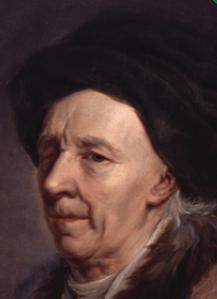
\includegraphics[scale=0.6]{euler.jpg}
  						\caption{Leonhard Euler (1707 - 1783)}
				\end{figure}

				Sa méthode repose sur la définition de la dérivée d'une fonction, pour une application $y : [a,b] \to \mathbb{R}^{m}$ dérivable en $x \in [a,b]$, on a l'expression de sa dérivée en $x$ :
				\[
					y'(x) = \lim_{t \to x} \frac{y(t) - y(x)}{t - x} = \lim_{h \to 0} \frac{y(x + h) - y(x)}{h} 
				\] 
				Pour $h$ proche de $0$, on a donc l'approximation suivante :
				\[
					y(x + h) \approx y(x) + hy'(x)
				\]
				Dans le cas du système $(S)$ à résoudre, on a $y'(x) = f(x, y(x))$.
				Ainsi,
				\[
					y(x + h) \approx y(x) + hf(x, y(x)) 
				\]
				Et donc, pour un pas maximal $h$ proche de $0$ :
				\[
					y(x_{k} + h_{k}) \approx y(x_{k}) + h_{k}f(x_{k}, y(x_{k})) 
				\]

				On en déduit donc une méthode de calcul de $y_{k+1}$ relativement correcte en posant $\forall k \in \llbracket 0, n-1 \rrbracket$ :
				\[
					y_{k+1} = y_{k} + h_{k}f(x_{k}, y_{k}) 
				\]
				i.e.
				\[
					\phi(x_{k}, y_{k}, h_{k}) = f(x_{k}, y_{k}) 
				\]
				Cette méthode est clairement consistante et stable théoriquement, elle est donc convergente.

			\subsection{Point-milieu}
				Le problème de la méthode d'Euler est qu'elle est d'ordre 1.
				Une solution serait de passer par un développement de Taylor, pour une application $y : [a,b] \to \mathbb{R}^{m}$ dérivable $p + 1$ fois en $x \in [a,b]$ et $y^{(p + 1)}$ bornée :
				\[
				\begin{aligned}
					y(x + h) & = \sum_{k = 0}^{p} \frac{h^{k}}{k!} y^{(k)}(x) + O(h^{p + 1}) \\
							 & = y(x) + hy'(x) + \frac{h^{2}}{2}y''(x) + … + \frac{h^{p}}{p!} y^{(p)}(x) + O(h^{p + 1}) \\
							 & = y(x) + hf(x, y(x)) + \frac{h^{2}}{2}\frac{df}{dx}(x,y(x)) + … + O(h^{p + 1})
				\end{aligned}
				\]

				Il devient nécessaire de calculer les dérivées partielles de $f$, qui sont difficiles à évaluer… par exemple, pour une méthode d'ordre 2 :
				\[
					y(x + h)  = y(x) + hf(x,y(x)) + \frac{h^{2}}{2}\frac{df}{dx}(x,y(x)) + O(h^{3})
				\]
				Et alors on doit calculer :
				\[
				\begin{aligned}
					\frac{df}{dx}(x,y(x)) & = \frac{\partial f}{\partial x}(x,y(x)) + \frac{\partial f}{\partial y}(x,y(x))\frac{dy}{dx}(x) \\
										  & = \frac{\partial f}{\partial x}(x,y(x)) + \frac{\partial f}{\partial y}(x,y(x)) f(x,y(x))
				\end{aligned}
				\]

				La méthode du point-milieu nous évite ce calcul fastidieux en centrant l'évaluation de la dérivée au point-milieu $x_{m} = \frac{x_{k} + x_{k+1}}{2}$ :
				\[
				\begin{aligned}
					y(x_{k} + h_{k}) & = y(x_{k+1}) \\
					 				 & = y(x_{m} + \frac{h_{k}}{2}) \\
					 				 & = y(x_{m}) + \frac{h_{k}}{2}y'(x_{m}) + \frac{h_{k}^{2}}{8}y''(x_{m}) + O(h_{k}^{3}) \\
				    y(x_{k}) & = y(x_{m} - \frac{h_{k}}{2}) \\
				    		 & = y(x_{m}) - \frac{h_{k}}{2}y'(x_{m}) + \frac{h_{k}^{2}}{8}y''(x_{m}) + O(h_{k}^{3}) \\ 
				\end{aligned}
				\]
				On en déduit :
				\[
				\begin{aligned}
					& y(x_{k+1}) - y(x_{k}) = h_{k}y'(x_{m}) + O(h_{k}^{3}) \\
					\Leftrightarrow \ & y(x_{k+1}) = y(x_{k}) + h_{k}f(x_{m}, y(x_{m})) + O(h_{k}^{3})
				\end{aligned}
				\]
				Or,
				\[
				\begin{aligned}
				    y(x_{m}) & = y(x_{k} + \frac{h_{k}}{2}) \\
				    		 & = y(x_{k}) + \frac{h_{k}}{2}y'(x_{k}) + O(h_{k}^{2}) \\ 
				    		 & = y(x_{k}) + \frac{h_{k}}{2}f(x_{k}, y(x_{k})) + O(h_{k}^{2}) \\ 
				\end{aligned}
				\]

				D'où l'expression de la méthode du point-milieu en posant $\forall k \in \llbracket 0, n-1 \rrbracket$ :
				\[
					y_{k+1} = y_{k} + h_{k}f\left(x_{k} + \frac{h_{k}}{2}, y_{k} + \frac{h_{k}}{2}f(x_{k}, y_{k})\right) 
				\]
				i.e.
				\[
					\phi(x_{k}, y_{k}, h_{k}) = f\left(x_{k} + \frac{h_{k}}{2}, y_{k} + \frac{h_{k}}{2}f(x_{k}, y_{k})\right)
				\]
				On peut montrer que cette méthode est d'ordre 2, ce qui est déjà plus intéressant.
				D'autres méthodes furent développées à la fin du \siecle{19} siècle, notamment la méthode de Heun, la méthode d'Euler modifiée.
				Mais c'est à l'aube du \siecle{20} siècle que des méthodes bien plus puissantes furent énoncées…

			\subsection{Méthodes de Runge-Kutta}
				En 1901, deux scientifiques allemands, Carl Runge et Martin Kutta, développèrent des méthodes de résolution numériques des EDO : les méthodes Runge-Kutta.
				Carl Runge était un physicien, mais c'est en faisant ses recherches sur les spectres atomiques qu'il développa ces méthodes pour résoudre des systèmes différentiels.
				Il pratiquait tellement les mathématiques que les physiciens le méprenait pour un mathématicien, et inversement.
				Kutta, lui, travaillait en mathématiques appliquées et apporta dans sa thèse une contribution très importante à la construction de ces méthodes encore utilisées aujourd'hui.
				\newpage
				\begin{figure}[!h]
 					\begin{minipage}[b]{.45\linewidth}
 						\centering
 							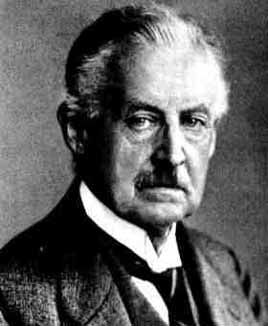
\includegraphics[scale=0.513]{runge.jpg}
 							\caption{Carl David Tolmé Runge (1856 - 1927)}
 					\end{minipage} \hfill
 					\begin{minipage}[b]{.45\linewidth}
 						\centering
 							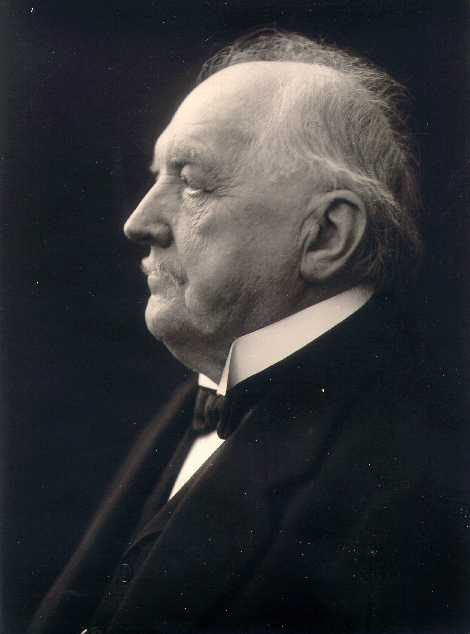
\includegraphics[scale=0.55]{kutta.jpg}
 							\caption{Wilhelm Martin Kutta (1867 - 1944)}
 					\end{minipage}
				\end{figure}

				Le principe des méthodes de Runge et Kutta repose sur la création de points intermédiaires $(x_{k,i})_{i \in \llbracket 1, r \rrbracket}$ pour chaque intervalle $[x_{k}, x_{k+1}]$ définis par : $x_{k,i} = x_{k} + \theta_{i}h_{k}$ avec $\theta_{i} \in [0,1]$.
				On se donne des coefficients réels $(a_{i,j})_{i,j \in \llbracket 1, r \rrbracket}$ et $(c_{i})_{i \in \llbracket 1, r \rrbracket}$.
				On définit alors :
				\[
					y_{k,i} = y_{k} + h_{k}\sum_{j = 1}^{r} a_{i,j}f(x_{k,j},y_{k,j})
				\]
				Et la suite $(y_{k})_{k \in \llbracket 0, n \rrbracket}$ par $y_{0}$ et :
				\[
					y_{k+1} = y_{k} + h_{k}\sum_{i = 1}^{r} c_{i}f(x_{k,i},y_{k,i})
				\]

				Depuis le travail de John Butcher, un mathématicien Néo-Zélandais reconnu pour son apport exceptionnel en analyse numérique, on visualise les coefficients d'une méthode de Runge-Kutta par le tableau suivant, aussi appelé tableau de Butcher :
				\begin{figure}[!h]
 					\begin{minipage}[b]{.45\linewidth}
 						\centering
 							\begin{tabular}{c|ccc}
								$\theta_1$ & $a_{11}$ & $\ldots$ & $a_{1r}$\\
								$\vdots$ & $\vdots$ & & $\vdots$ \\
								$\theta_r$ & $a_{r1}$ & $\ldots$ & $a_{rr}$\\
								\hline
								&$c_1$ & $\ldots$ & $c_r$
							\end{tabular}
 							\caption{Tableau de Butcher}
 					\end{minipage} \hfill
 					\begin{minipage}[b]{.45\linewidth}
 						\centering
 							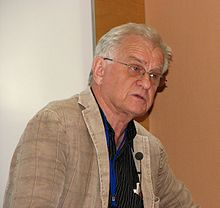
\includegraphics[scale=0.3]{butcher.jpg}
 							\caption{John Charles Butcher (1933)}
 					\end{minipage}
				\end{figure}

				Selon la valeur des coefficients de $A$, on peut avoir une méthode implicite ou explicite.
				En particulier, si $A$ est triangulaire inférieure à diagonale nulle, on retrouve bien une méthode explicite et :
				\[
					\phi(x_{k}, y_{k}, h_{k}) = \sum_{i = 1}^{r} c_{i}f\left(x_{k} + \theta_{i}h_{k}, y_{k} + h_{k}\sum_{j = 1}^{i - 1} a_{i,j}f(x_{k,j},y_{k,j})\right)
				\]
				On peut montrer que toutes les méthodes de Runge-Kutta explicites sont stables théoriquement, il suffit alors de trouver les bons coefficients pour avoir la convergence.

				En fait, les méthodes de Runge-Kutta généralisent des méthodes déjà connues.
				Par exemple, pour les méthodes de Euler et du point-milieu on a les tableaux de Butcher suivants :
				\begin{figure}[!h]
 					\begin{minipage}[b]{.45\linewidth}
 						\centering
 							\begin{tabular}{c|c}
								$0$ & $0$\\
								\hline
								&$1$
							\end{tabular}
 							\caption{Méthode d'Euler}
 					\end{minipage} \hfill
 					\begin{minipage}[b]{.45\linewidth}
 						\centering
 							\begin{tabular}{c|cc}
 								$0$ & $0$ & $0$\\
								$1/2$ & $1/2$ & $0$\\
								\hline
								&$0$ & $1$
							\end{tabular}
 							\caption{Méthode du point-milieu}
 					\end{minipage}
				\end{figure}

				Le grand intérêt est que l'on peut alors construire des méthodes d'ordre $p$ en trouvant les coefficients adéquats, il suffit d'avoir :
				\[
					\forall j \in \llbracket 0, p-1 \rrbracket, \ \frac{\partial^{j}\phi}{\partial h^{j}}(x,y(x),0) = \frac{1}{j+1}f^{(j)}(x,y(x))  
				\]
				i.e. pour une méthode d'ordre 1 (et donc consistante) :
				\[
					\sum_{i = 1}^{r} c_{i} = 1
				\]
				Pour une méthode d'ordre 2, il nous suffit d'avoir la condition de la méthode d'ordre 1 et :
				\[
					\frac{\partial\phi}{\partial h}(x,y(x),0) = \frac{1}{2}\frac{df}{dx}(x,y(x))  
				\]
				i.e.
				\[
					\sum_{i = 1}^{r} c_{i}\theta_{i}\frac{\partial f}{\partial x}(x, y(x)) + \sum_{i = 1}^{r} c_{i}\sum_{j = 1}^{i-1}a_{i,j}f(x,y(x))\frac{\partial f}{\partial y}(x, y(x)) = \frac{1}{2}\left(\frac{\partial f}{\partial x}(x,y(x)) + \frac{\partial f}{\partial y}(x,y(x)) f(x,y(x))\right)
				\]

				En ayant le même raisonnement et avec beaucoup de calculs, on peut trouver des conditions pour une méthode d'ordre $p$ :
				\begin{figure}[!h]
					\centering
						\begin{tabular}{|l|c|r|}
  							\hline
  							p & conditions \\
  							\hline
  							1 & $\sum_{i = 1}^{r} c_{i} = 1$ \\
  							\hline
  							2 & $\left\{
  									\begin{array}{rcl}
  										\sum \limits_{i = 1}^{r} c_{i}\theta_{i} & = & \frac{1}{2} \\
  										\sum \limits_{i = 1}^{r}\sum \limits_{j = 1}^{i-1} c_{i}a_{i,j} & = & \frac{1}{2}
  									\end{array}
  								\right.$ \\
  							\hline
  							3 & … \\
						\end{tabular}
						\caption{Les conditions à satisfaire pour une méthode d'ordre $p$}
				\end{figure}

				À mesure que l'ordre augmente, il devient de plus en plus difficile de trouver de bons coefficients étant donné que le nombre de conditions devient très élevé (58 conditions pour $p = 5$).
				Au \siecle{20} siècle, les mathématiciens ont pu assister à une véritable course à la recherche d'une méthode ayant  le plus grand ordre possible : la méthode la plus efficace étant d'ordre $2$ en 1895 (Runge), $5$ en 1901 (Kutta) et $10$ en 1978 (Hairer).


		\section{La méthode de Runge-Kutta $RK_{34}$}
			La méthode de Runge-Kutta $RK_{34}$ est une méthode dite à \og formules emboîtées \fg. 

			\subsection{Les méthodes de Runge et Kutta à formules emboîtées}
				On dira qu'un couple $RK_{pp'}$ ($p' \geq p + 1$) est une méthode de Runge-Kutta à formules emboîtées si elle est formée par une méthode de Runge-Kutta d'ordre $p$ complétée par une ligne et une colonne afin d'obtenir une méthode d'ordre $p'$.
				\begin{figure}[!h]
				 	\centering
 						\begin{tabular}{c|cccc}
							$\theta_1$ & $a_{11}$ & $\ldots$ & $a_{1r}$ & $\textcolor{green}{0}$\\
							$\vdots$ & $\vdots$ & & $\vdots$ & $\textcolor{green}{\vdots}$ \\
							$\theta_r$ & $a_{r1}$ & $\ldots$ & $a_{rr}$ & $\textcolor{green}{0}$\\
							$\textcolor{green}{1}$ & $c_1$ & $\ldots$ & $c_r$ & $\textcolor{green}{0}$\\
							\hline
							& $\textcolor{green}{c'_1}$ & $\textcolor{green}{\ldots}$ & $\textcolor{green}{c'_r}$ & $\textcolor{green}{c'_{r+1}}$
						\end{tabular}
 						\caption{Tableau de Butcher d'une méthode $RK_{pp'}$}
				\end{figure}

				Dans le cas de la méthode $RK_{34}$, il s'agit donc d'une méthode de Runge-Kutta d'ordre $3$ complétée par une méthode d'ordre $4$.

			\subsection{Méthodes de contrôle du pas}
				Le grand intérêt des méthodes $RK_{pp'}$ est qu'elles permettent un contrôle de l'erreur de consistance pour l'empêcher de dépasser un certain seuil.
				Si l'on suppose que l'on utilise une méthode d'ordre $p$ pour calculer $(y_{k})_{k \in \llbracket 0,n \rrbracket}$ : 
				\[
					y_{k+1} = y_{k} + h_{k}\phi(x_{k}, y_{k}, h_{k})
				\]
				On a donc l'expression suivante de l'erreur de consistance :
				\[
					\epsilon_{k} = y(x_{k+1}) - y(x_{k}) - h_{k}\phi(x_{k}, y(x_{k}), h_{k})
				\]
				On suppose que l'on utilise une autre méthode d'ordre $p'$ telle que $p' \geq p + 1$.
				On aura aussi une expression de l'erreur de consistance commise avec cette méthode :
				\[
					\epsilon_{k}^{*} = y(x_{k+1}) - y(x_{k}) - h_{k}\phi^{*}(x_{k}, y(x_{k}), h_{k}) = O(h_{k}^{p+2})
				\]
				D'où :
				\[
					\epsilon_{k} = \epsilon_{k}^{*} + h_{k}\left(\phi^{*}(x_{k}, y(x_{k}), h_{k}) - \phi(x_{k}, y(x_{k}), h_{k})\right)
				\]

				On ne sait pas calculer $y(x_{k})$, mais on peut utiliser un développement limité au premier ordre pour exprimer $\phi$ en fonction de $y_{k}$; il existe $\bar{y_{k}}$ compris entre $y_{k}$ et $y(x_{k})$ tel que :
				\[
				\begin{aligned}
					\epsilon_{k} & = \epsilon_{k}^{*} + h_{k}\left(\phi^{*}(x_{k}, y_{k}, h_{k}) - \phi(x_{k}, y_{k}, h_{k}) + (y(x_{k}) - y_{k})\left(\frac{\partial \phi^{*}}{\partial y}(x_{k}, \bar{y_{k}}, h_{k}) - \frac{\partial \phi}{\partial y}(x_{k}, \bar{y_{k}}, h_{k})\right)\right) \\
								 & = \epsilon_{k}^{*} + h_{k}\left(\phi^{*}(x_{k}, y_{k}, h_{k}) - \phi(x_{k}, y_{k}, h_{k}) + (y(x_{k}) - y_{k})\left(\frac{\partial \phi^{*}}{\partial y}(x_{k}, \bar{y_{k}}, 0) - \frac{\partial \phi}{\partial y}(x_{k}, \bar{y_{k}}, 0) + O(h_{k})\right)\right)
				\end{aligned}
				\]
				Or, par consistance et comme $y(x_{k}) - y_{k} = O(h_{k}^{p})$ :
				\[
				\begin{aligned}
					\epsilon_{k} & = \epsilon_{k}^{*} + h_{k}\left(\phi^{*}(x_{k}, y_{k}, h_{k}) - \phi(x_{k}, y_{k}, h_{k}) + O(h_{k}^{p})\left(\frac{\partial f}{\partial y}(x_{k}, \bar{y_{k}}) - \frac{\partial f}{\partial y}(x_{k}, \bar{y_{k}}) + O(h_{k})\right)\right) \\
								 & = \epsilon_{k}^{*} + h_{k}\left(\phi^{*}(x_{k}, y_{k}, h_{k}) - \phi(x_{k}, y_{k}, h_{k}) + O(h_{k}^{p+1})\right) \\
								 & = O(h_{k}^{p+2}) + h_{k}\left(\phi^{*}(x_{k}, y_{k}, h_{k}) - \phi(x_{k}, y_{k}, h_{k})\right)\\
								 & \approx h_{k}\left(\phi^{*}(x_{k}, y_{k}, h_{k}) - \phi(x_{k}, y_{k}, h_{k})\right)
				\end{aligned}
				\]

				Finalement, on a bien une bonne approximation calculable $\bar{\epsilon_{k}}$ de $\epsilon_{k}$.
				Dans le cas d'une méthode de Runge-Kutta emboîtée, on a :
				\[
				\begin{aligned}
					\bar{\epsilon_{k}} & = h_{k}\left(\phi^{*}(x_{k}, y_{k}, h_{k}) - \phi(x_{k}, y_{k}, h_{k})\right)\\
								 		 & = h_{k}\left(\sum_{i = 1}^{r} (c'_{i} - c_{i})f(x_{k,i}, y_{k,i}) + c'_{r+1}f(x_{k,r+1}, y_{k,r+1})\right)\\
								 		 & = h_{k}\left(\sum_{i = 1}^{r} (c'_{i} - c_{i})f(x_{k,i}, y_{k,i}) + c'_{r+1}f\left(x_{k} + \theta_{r+1}h_{k}, y_{k} + \sum_{j=1}^{r+1}a_{r+1,j}f(x_{k,j}, y_{k,j})\right)\right)\\
								 		 & = h_{k}\left(\sum_{i = 1}^{r} (c'_{i} - c_{i})f(x_{k,i}, y_{k,i}) + c'_{r+1}f(x_{k+1}, y_{k+1})\right)
				\end{aligned}
				\]
				
				Maintenant, si l'on souhaite avoir une erreur de consistance en dessous d'un certain seuil $\delta$, il suffit de comparer à 1 ce terme : 
				\[
					e = \frac{|\bar{\epsilon_{k}}|}{\delta}
				\]

				\begin{itemize}
					\item si $e > 1$ alors il faut réduire le pas;
					\item si $e < 1$ alors il faut prendre un pas plus grand pour limiter les calculs;
					\item si $e = 1$ alors on a un pas optimal.
				\end{itemize}
				On aimerait donc modifier le pas après chaque test de telle sorte qu'il soit optimal.
				Or, on sait que pour $h_{k}$ au voisinage de $0$ :
				\[
					e \approx Ch_{k}^{p+1}
				\]
				Et donc
				\[
					C \approx \frac{e}{h_{k}^{p+1}}
				\]
				Et, pour un pas optimal :
				\[
					e = 1 \approx Ch_{k_{opt}}
				\]
				Finalement, on pourrait prendre :
				\[
					h_{k_{opt}} = h_{k}\left(\frac{1}{e}\right)^{\frac{1}{p+1}}
				\]
				Mais on préfère se donner une petite marge de sécurité :
				\[
					h_{k_{opt}} = 0.9h_{k}\left(\frac{1}{e}\right)^{\frac{1}{p+1}}
				\]\\

			\subsection{La méthode de Runge-Kutta $RK_{34}$}
				Le tableau de Butcher de la méthode que nous étudierons dans ce projet est le suivant :
				\begin{figure}[!h]
				 	\centering
 						\begin{tabular}{c|ccccc}
							$0$ & $0$ & $0$ & $0$ & $0$ & $\textcolor{green}{0}$\\
							$2/7$ & $2/7$ & $0$ & $0$ & $0$ & $\textcolor{green}{0}$ \\
							$4/7$ & $-8/35$ & $4/5$ & $0$ & $0$ & $\textcolor{green}{0}$\\
							$6/7$ & $29/42$ & $-2/3$ & $5/6$ & $0$ & $\textcolor{green}{0}$\\
							$\textcolor{green}{1}$ & $1/6$ & $1/6$ & $5/12$ & $1/4$ & $\textcolor{green}{0}$\\
							\hline
							& $\textcolor{green}{11/96}$ & $\textcolor{green}{7/24}$ & $\textcolor{green}{35/96}$ & $\textcolor{green}{7/48}$ & $\textcolor{green}{1/12}$
						\end{tabular}
 						\caption{Tableau de Butcher de la méthode $RK_{34}$}
				\end{figure}

				Vérifions que la méthode d'ordre 3 non complétée est bien consistante :
				\[\begin{aligned}
					\sum_{i = 1}^{r} c_{i} & = \frac{1\times2}{6\times2} + \frac{1\times2}{6\times2} + \frac{5}{12} + \frac{1\times3}{4\times3}\\
										   & = 1
				\end{aligned}\]
				Elle est aussi bien d'ordre $2$ :
				\[\begin{aligned}
					\sum \limits_{i = 1}^{r} c_{i}\theta_{i} & = 0 + \frac{2 \times 1}{7 \times 6} + \frac{4 \times 5}{7 \times 12} + \frac{6 \times 1}{7 \times 4}\\
															 & = \frac{2\times2}{42\times2} + \frac{10\times2}{42\times2} + \frac{6\times3}{28\times3}\\
										   					 & = \frac{1}{2}\\
				\end{aligned}\]
				Et,
				\[\begin{aligned}
					\sum \limits_{i = 1}^{r}\sum \limits_{j = 1}^{i-1} c_{i}a_{i,j} & = \frac{1 \times 2}{6 \times 7} + \frac{5}{12}(-\frac{8}{35} + \frac{4 \times 7}{5 \times 7}) + \frac{1}{4}(\frac{29}{42} - \frac{2 \times 14}{3 \times 14} + \frac{5 \times 7}{6 \times 7}) \\
					& = \frac{2}{42} + \frac{5}{12}\frac{20}{35} + \frac{1}{4}\frac{36}{42} \\
					& = \frac{4}{84} + \frac{20}{84} + \frac{18}{84} \\
					& = \frac{1}{2}
				\end{aligned}\]
				On peut aussi vérifier qu'elle est bien d'ordre 3.
				Nous ne ferons pas ici ce calcul, car le nombre de conditions à vérifier est important.

				Vérifions que la méthode emboîtée d'ordre 4 est bien consistante :
				\[\begin{aligned}
					\sum_{i = 1}^{r+1} c'_{i} & = \frac{11}{96} + \frac{7 \times 4}{24 \times 4} + \frac{35}{96} + \frac{7 \times 2}{48 \times 2} + \frac{1\times 8}{12 \times 8}\\
										   & = 1
				\end{aligned}\]
				De même, cette méthode est bien d'ordre $2$ :
				\[\begin{aligned}
					\sum \limits_{i = 1}^{r+1} c'_{i}\theta_{i} & = 0 + \frac{2 \times 7}{7 \times 24} + \frac{4 \times 35}{7 \times 96} + \frac{6 \times 7}{7 \times 48} + \frac{1}{12}\\
															 & = \frac{2}{24} + \frac{5}{24} + \frac{3}{24} + \frac{2}{24}\\
										   					 & = \frac{1}{2}\\
					\sum \limits_{i = 1}^{r+1}\sum \limits_{j = 1}^{i-1} c'_{i}a_{i,j} & = \frac{7 \times 2}{24 \times 7} + \frac{35}{96}(-\frac{8}{35} + \frac{4 \times 7}{5 \times 7}) + \frac{7}{48}(\frac{29}{42} - \frac{2 \times 14}{3 \times 14} + \frac{5 \times 7}{6 \times 7}) + \frac{1}{12}(\frac{1\times 2}{6 \times 2} + \frac{1\times 2}{6 \times 2} + \frac{5}{12} + \frac{1 \times 3}{4\times 3}) \\
					& = \frac{2}{24} + \frac{35}{96}\frac{20}{35} + \frac{7}{48}\frac{36}{42} + \frac{1}{12}\times1 \\
					& = \frac{8}{96} + \frac{20}{96} + \frac{12}{96} + \frac{8}{96} \\
					& = \frac{1}{2}
				\end{aligned}\]
				On peut vérifier que la méthode est bien d'ordre 3, puis d'ordre 4…



	\chapter{Implémentation de la méthode $RK_{34}$ en C}
		Dans cette partie, nous allons développer un programme C pour pouvoir calculer la suite de points approximant la solution de $(S)$.
		On adoptera d'abord une démarche structurée pour écrire en pseudo-langage toutes les opérations qui seront nécessaires au bon fonctionement de la méthode.
		Ensuite, nous nous intéresserons au coût (en terme d'opérations) engendré par tous ces calculs.
		Puis, nous parlerons rapidement des erreurs d'approximation machine qui viennent s'ajouter aux erreurs générées par la méthode et qui seront à prendre en compte dans la suite de ce projet.
		Enfin, nous présenterons rapidement le programme réalisé.

		\section{L'algorithme}
			On se donne d'emblée un tableau constant $rk34$ de taille $6\times6$ qui contient tout les coefficients de la méthode (i.e. le tableau de Butcher présenté précédemment).

			Nous avons vu que la méthode $RK_{34}$ sert à utiliser un pas adaptatif pour contrôler l'erreur de consistance; ainsi on peut affirmer que le nombre de points générés par la méthode ne peut pas être \og prédit \fg{} et dépendra de la fonction $f$ et du seuil choisi.
			On peut donc remarquer que trois boucles imbriquées seront nécessaires au bon fonctionnement de la méthode :
			\begin{enumerate}
				\item Une boucle principale indéterministe dont la condition d'arrêt sera de savoir si l'abscisse $x_{k}$ calculée a dépassé la borne $b$ de l'intervalle $[a,b]$.
				\item Une boucle déterministe que l'on fera dépendre d'une variable $i$, dans laquelle les points intérmédiaires $(x_{k,i},y_{k,i})$ seront calculés.
				\item Une dernière boucle déterministe qui dépendra d'une variable $j$, à l'intérieur de laquelle se déroulera le calcul d'un $y_{k,i}$ ($i$ fixé).
			\end{enumerate}

			Notre première idée était de stocker les points calculés (i.e. les $(x_{k},y_{k})$) dans un tableau au fur et à mesure de l'exécution du programme.
			On a vu que, si l'on veut contrôler l'erreur, il est impossible de \og prédire \fg{} la taille de ce tableau à l'avance.
			Nous avons donc, dans un premier temps, réalisé un programme en Fortran en allouant dynamiquement ce tableau.
			Le problème est que cette façon de concevoir la méthode est couteuse en mémoire et en complexité (il faut, à chaque fois que l'on dépasse la taille initiale du tableau, réallouer un espace mémoire plus grand et déplacer toutes les données).
			Nous nous sommes alors aperçus qu'il ne nous était pas nécéssaire de conserver les points calculés en mémoire, mais plutôt de les sauvegarder au fur et à mesure dans un fichier, ce qui est moins couteux.

			Il nous a donc semblé logique d'utiliser des variables locales $x$ et $y$ chargées de contenir respectivement l'abscisse et l'ordonnée du point $(x_{k},y_{k})$ en cours de traitement, puis de les sauvegarder une fois le calcul et l'affectation de $x_{k+1}$ et $y_{k+1}$ effectué.
			Sachant qu'il est inutile de conserver en mémoire les points intérmédiaires $(x_{k,i},y_{k,i})$, nous avons aussi utilisé deux variables locales $xtmp$ et $ytmp$ pour les stocker au fur et à mesure.
			Pour limiter le nombre d'appels de la fonction $f$, nous avons utilisé un tableau $fct$ chargé de conserver les valeurs des $f(x_{k,i}, y_{k,i})$ en mémoire (à chaque nouvelle itération dans la boucle principale, ces valeurs laissent place aux nouvelles).

			Pour simplifier l'algorithme, nous avons affiché au fur et à mesure les points $(x_{k},y_{k})$, mais dans notre programme C ces points sont sauvegardés dans un fichier (comme le pas et l'erreur).

			\begin{figure}[!h]
				\begin{algorithme}
				    \procedure{rungeKutta34}{\paramEntree{a, b, y0, seuil : \reel, f : \typeFonction{x,y : \reel}{\reel}}}{
				    x, y, h, xtmp, ytmp, phi3, phi4, erreur, e : \reel, fct : \tableauUneDimension{1…4}{de }{\reel}, i, j : \entier
				    \constante{rk34}{\tableauDeuxDimensions{1…6}{1…6}{de}{\reel}}
				    \constante{NINIT}{10000}}{
				        \affecter{x}{a}
				        \affecter{y}{y0}
				        \affecter{h}{(b-a)/(NINIT)}
				        \ecrire{x,y}
				        \tantque{(x < b)}{
				            \affecter{xtmp}{0}
				            \affecter{ytmp}{0}
				            \affecter{phi3}{0}
				            \affecter{phi4}{0}
				            \pour{i}{1}{4}{}{
				                \affecter{xtmp}{x + h*rk34[i][1]}
				                \affecter{ytmp}{y}
				                \pour{j}{2}{i}{}{
				                    \affecter{ytmp}{ytmp + rk34[i][j]*fct[j-1]}
				                }
				                \affecter{ytmp}{y + h*ytmp}
				                \affecter{fct[i]}{f(xtmp, ytmp)}
				                \affecter{phi3}{phi3 + rk34[5][i+1]*fct[i]}
				                \affecter{phi4}{phi4 + rk34[6][i+1]*fct[i]}
				            }
				            \affecter{x}{x + h}
				            \affecter{y}{y + h*phi3}
				            \affecter{phi4}{phi4 + rk34[6][6]*f(x,y)}
				            \affecter{erreur}{h*(phi4 - phi3)}
				           	\affecter{e}{abs(erreur/seuil)}
				            \sialorssinon{(e > 1) et (e > 0)}{
				            	\affecter{h}{0.9*h*(1/e$)^{1/4}$}
				            }{
				            	\sialors{(e < 0.9) et (e > 0)}{
				                	\affecter{h}{0.9*h*(1/e$)^{1/4}$}
				            	}
				            	\sialors{(x $\leq$ b)}{
				            		\ecrire{x,y}
				            	}
				            }
				        }
				    }
				\end{algorithme}
				\caption{L'algorithme de la méthode $RK_{34}$}
			\end{figure}
			\newpage

		\section{La complexité}
			Comme nous l'avons spécifié précédemment, on ne peut pas prédire le nombre d'itérations réalisées dans la boucle principale sans connaitre la fonction $f$ et le seuil rentré par l'utilisateur.
			On appellera donc $\alpha = \alpha_{f,seuil}$ ce nombre d'itérations.
			On néglige le cout engendrée par l'affectation et on considérera l'appel d'une fonction comme étant une opération (ce qui est, normalement, plus couteux).

			Dans la boucle principale, on compte :
			\begin{itemize}
				\item un certain nombre d'opérations dans la boucle $i$ : $n_{i}$;
				\item une somme pour le calcul de $x$;
				\item une somme et une multiplication pour le calcul de $y$;
				\item une somme, une multiplication et un appel de fonction pour la fin du calcul de $phi4$, puis une multiplication et une somme pour le calcul de $erreur$;
				\item une divison pour le calcul de $e$;
				\item on suppose que l'on change $h$ à chaque fois et donc que l'on effectue deux multiplication et un appel de fonction (pour la puissance $1/4$).
			\end{itemize}
			Donc $n_{i} + 12$ opérations.

			Dans la boucle $i$, on a :
			\begin{itemize}
				\item $i-1$ sommes et $i-1$ multiplications dans la boucle $j$;
				\item une somme et une multiplication pour le calcul de $xtmp$;
				\item une somme et une multiplication pour le calcul de $ytmp$;
				\item un appel de la fonction $f$;
				\item une somme et une multiplication pour le calcul de $phi3$;
				\item une somme et une multiplication pour le calcul de $phi4$.
			\end{itemize}
			Donc $n_{i} = \sum_{i = 1}^{4} (2i + 7) = 48$ opérations.

			On a donc $60$ opérations à chaque exécution de la boucle principale, donc $60 \alpha$ opérations en tout.
			Par exemple, dans le cas de la même méthode à pas constant, on a $60n$ opérations pour $n$ points à calculer.

		\section{Présentation du programme C}
			Nous avons implémenté la méthode en langage C, en prenant soin de copier les valeurs des points, de l'erreur de consistance et du pas dans des fichiers dans un dossier $data$ pour pouvoir les utiliser.
			De plus, nous avons aussi codé la même méthode à pas constant pour pouvoir comparer les résultats plus tard.
			Dans le programme suivant on a choisi $y' = y$, il suffit de modifier la valeur de retour de $f$ pour pouvoir utiliser notre programme sur une autre équation différentielle.
			Si nous avions eu plus de temps, nous aurions souhaité passer la fonction $f$ en paramètre du programme en utilisant une librairie d'évaluation d'expression mathématiques (comme muParser, par exemple).
			\lstinputlisting{"../Programme/src/main.c"}

		\section{Précision machine et approximations}
			Il est nécessaire de souligner que les solutions obtenues ne sont pas toujours exactes mais approximées. 
			En effet, outre les erreurs dûes aux methodes de résolutions, il existe également des erreurs dues à la machine.
			Nos ordinateurs disposent d'une capacité de représentation finie : d'une part, certains nombres sont trop petits pour être représentés, et de la même manière il existe des nombres qui dépassent cette capacité. 
			Dans ce cas là, on parlera alors respectivement d'\emph{underflow} et d'\emph{overflow}. 
			Un \emph{overflow} provoquera la représentation du nombre comme \emph{infinity} et arrêtera directement l'éxecution, tandis qu'un \emph{underflow} sera arrondi à zéro.
			
			D'autre part la représentation informatique des réels repose sur une expression binaire (i.e. en base $2$) de ces nombres.
			Ainsi, des nombres ayant une valeur exacte dans une base peut avoir une valeur arrondie dans une autre. 
			La machine effectue donc des approximations afin de pouvoir les représenter. 
			On a l'exemple de $0.1$ qui en décimal aura une expression finie tandis qu'en binaire aura une représentation périodique infini.
			
			Enfin il est important de souligner que l'arrondi d'un réel dans un programme donné peut amener à une accumulation d'erreurs. 
			Une erreur d'abord non significative aura de grandes répercutions du fait du nombre important de fois où elle est réalisée, on assistera alors à une dégradation progressive du résultat.

	\chapter{Application de la méthode $RK_{34}$ sur des exemples}
		Nous allons ici appliquer la méthode $RK_{34}$ et la méthode $RK_{3}$ sur des exemples concrets pour tester leur efficacité.
		On se donnera des EDO resolvables pour pouvoir calculer l'erreur commise par la méthode : $(e_{k})_{k \in \llbracket 0,n \rrbracket} = (|y_{k} - y(x_{k}|)_{k \in \llbracket 0,n \rrbracket}$.
	
		\section{Quelques exemples intéressants}

			\subsection{Exponentielle}
				On se donne $f(x,y) = y$.

				\subsubsection{Résolution directe}
				
				On a :
				\[\begin{aligned}
					y' = y \\
					& \Leftrightarrow \frac{dy}{dt} = y
				\end{aligned}\]

				On suppose $y \neq 0$,

				\[\begin{aligned}
					\frac{dy}{y} = dt
					& \Leftrightarrow \int_{a}^{x} \frac{dy}{y} =\int_{a}^{x} dt \\
					& \Leftrightarrow ln(|y|)-ln(|y_0|) = x-a \\
					& \Leftrightarrow ln(|\frac{y}{y_0}|)=x-a \\
					& \Leftrightarrow \frac{y(x)}{y_0} = e^{x-a} \\
					& \Leftrightarrow y(x)=y_{0}e^{x-a}
				\end{aligned}\]

				\subsubsection{Application de la méthode}
					Dans un premier temps , nous avons étudié les valeurs de la solution pour la valeur initiale $y_0=1$ puis celles pour $y_0=1000$.

					\begin{figure}[!h]
						\centering
  							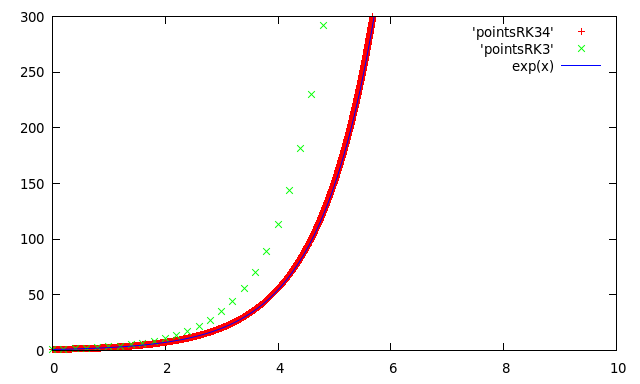
\includegraphics[scale=0.5]{courbe.png}
  							\caption{Pour $y_0=1$ sur l'intervalle $[0,10]$, seuil de $10^{-5}$, pas de $50$}
					\end{figure}
	
					\begin{figure}[!h]
						\centering
  							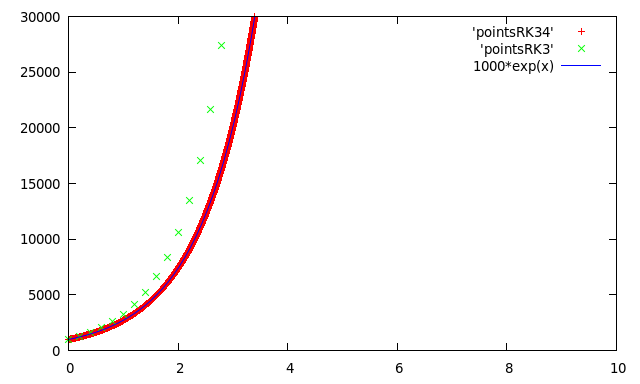
\includegraphics[scale=0.5]{courbexcf.png}
  							\caption{Pour $y_0=1000$ sur l'intervalle $[0,10]$, seuil de $10^{-5}$, pas de $50$}
					\end{figure}
					\newpage

					Puis, nous nous sommes intéressés à la comparaison de l'erreur de consistance selon la méthode utilisée :
					\begin{figure}[!h]
						\centering
  							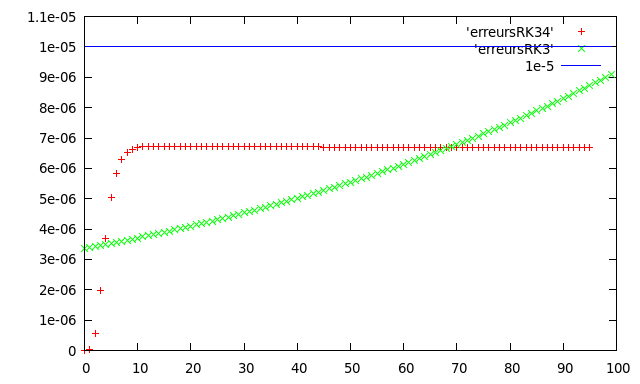
\includegraphics[scale=0.5]{erreurExpCroissante.png}
  							\caption{Pour $y_0=1$ sur l'intervalle $[0,1]$, seuil de $10^{-5}$, pas de $100$}
					\end{figure}
					\newpage

					On remarque que l'erreur de consistance croit pour la méthode à pas constant, alors qu'elle se stabilise pour la méthode à pas adaptatif.
					On remarque aussi que l'erreur de consistance est bien en dessous du seuil fixé, voir trop en dessous.
					Cela est du au facteur $0.9$ que l'on s'est donné par sécurité dans le calcul du $h_{{k}_{opt}}$.
					En enlevant cette sécurité, on a l'erreur de consistance suivante :
					\begin{figure}[!h]
						\centering
  							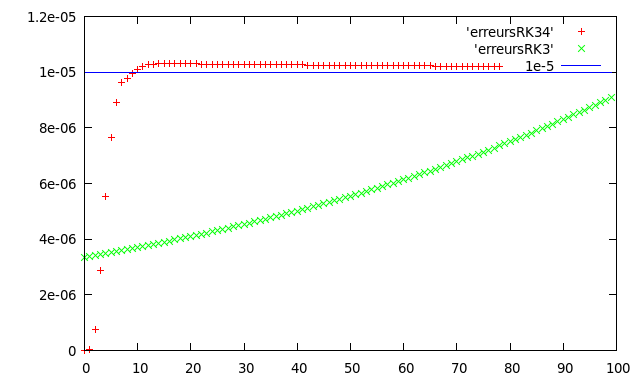
\includegraphics[scale=0.5]{erreurExpCroissanteSansSecurite.png}
  							\caption{Pour $y_0=1$ sur l'intervalle $[0,1]$, seuil de $10^{-5}$, pas de $100$}
					\end{figure}

					Cette erreur est clairement au dessus du seuil fixé, on voit donc bien l'intérêt de ce facteur de sécurité.
					\newpage

					Nous avons l'erreur réelle suivante pour la méthode $RK_{34}$, qui croit fortement et dépasse clairement le seuil de l'erreur de consistance :
					\begin{figure}[!h]
						\centering
  							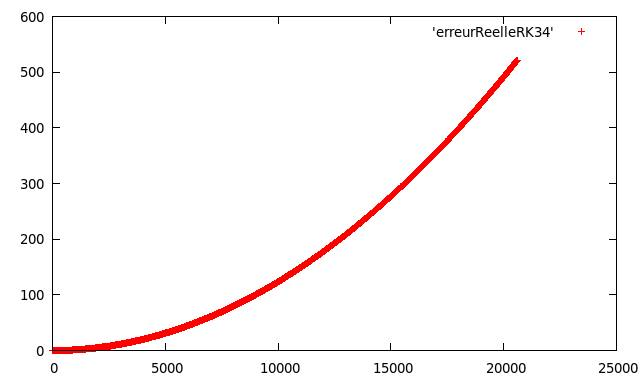
\includegraphics[scale=0.5]{erreurReelleExpCroissante.jpg}
  							\caption{Pour $y_0=1$ sur l'intervalle $[0,10]$, seuil de $10^{-5}$, pas de $50$}
					\end{figure}

					Pour la méthode $RK_{3}$, l'erreur explose :
					\begin{figure}[!h]
						\centering
  							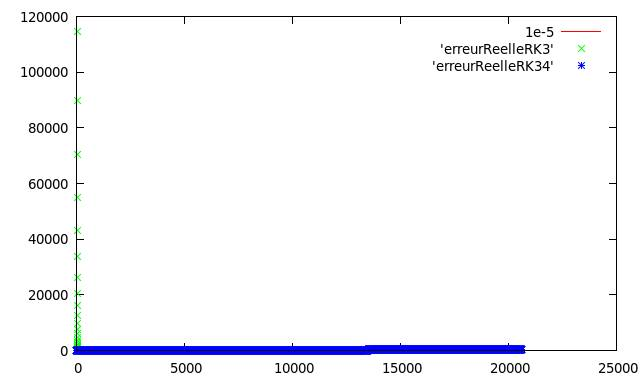
\includegraphics[scale=0.5]{erreurReelleExpCroissante2.jpg}
  							\caption{Pour $y_0=1$ sur l'intervalle $[0,10]$, seuil de $10^{-5}$, pas de $50$}
					\end{figure}


				\subsubsection{Comparaison des résultats}
					On a pu montré ici que la méthode $RK_{34}$ était bien plus efficace dans le sens où elle contient bien mieux l'erreur de consistance et l'erreur réelle.
					On remarque tout de même une perte d'efficacité de la méthode pour une fonction dont la croissance est aussi démusurée que celle de l'exponentielle.

			\subsection{Exponentielle décroissante}
				On s'intéresse ici à $f(x,y) = -y$.

				\subsubsection{Résolution directe}
					De la même manière que précédemment, nous retrouvons :
					\[
						y(x) = y_{0}e^{-(x-a)}
					\]

				\subsubsection{Application de la méthode}
					Ici, nous utilisons les mêmes valeurs initiales que précédemment :

					\begin{figure}[!h]
						\centering
  							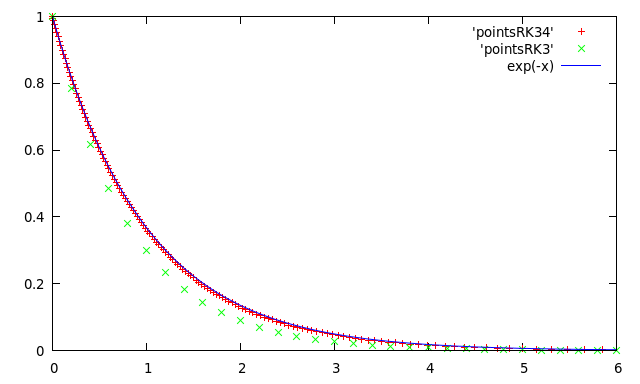
\includegraphics[scale=0.5]{exp1.png}
  							\caption{Pour $y_0=1$ sur l'intervalle $[0,10]$, seuil de $10^{-5}$, pas de $50$}
					\end{figure}
	
					\begin{figure}[!h]
						\centering
  							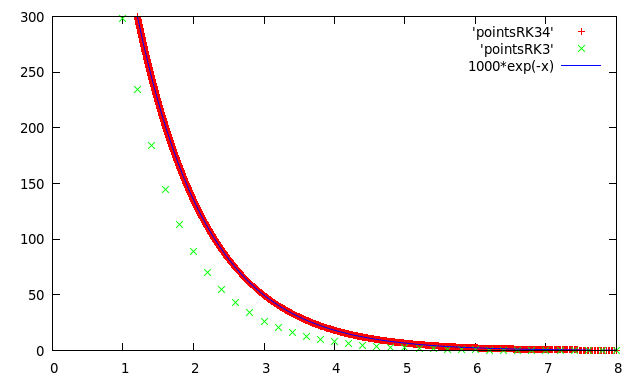
\includegraphics[scale=0.5]{1000exp2.png}
  							\caption{Pour $y_0=1000$ sur l'intervalle $[0,10]$, seuil de $10^{-5}$, pas de $50$}
					\end{figure}
					\newpage

					Ce qui donne, pour l'erreur de consistance :
					\begin{figure}[!h]
						\centering
  							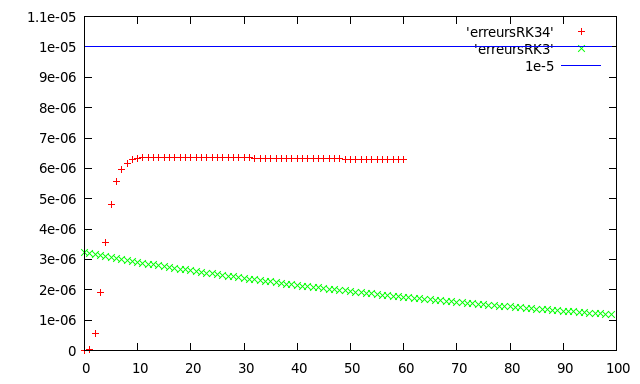
\includegraphics[scale=0.5]{erreurExpDecroissante.png}
  							\caption{Pour $y_0=1$ sur l'intervalle $[0,1]$, seuil de $10^{-5}$, pas de $100$}
					\end{figure}

					On remarque que l'erreur de consistance décroit pour la méthode à pas constant, alors qu'elle se stabilise pour la méthode à pas adaptatif.

					Concernant l'erreur réelle, on a :
					\begin{figure}[!h]
						\centering
  							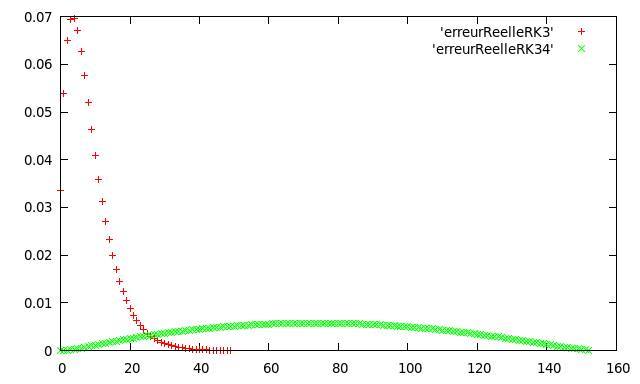
\includegraphics[scale=0.5]{erreurReelleExpDecroissante.jpg}
  							\caption{Pour $y_0=1$ sur l'intervalle $[0,10]$, seuil de $10^{-5}$, pas de $50$}
					\end{figure}
					\newpage

				\subsubsection{Comparaison des résultats}
					On remarque que l'erreur réelle est ici mal maitrisée par la méthode adaptatif : par un souci d'optimisation, celle-ci met un certain temps à atteindre une erreur aussi faible que celle à pas constant.
					Mais, la méthode à pas constant n'est pas très intéressante car l'erreur est très élevée puis décroit, alors que $RK_{34}$ nous offre un certain contrôle.

			\subsection{Ça oscille ici}
				On se propose d'étudier $f(x,y) = \frac{1}{x^{2}}sin\left(\frac{1}{x}\right)$.

				\subsubsection{Résolution directe}
					On commence par remarquer que :
					\[
						\left(cos(\dfrac{1}{x})\right)' = \frac{1}{x^{2}}sin\left(\frac{1}{x}\right)
					\]

					D'où :
					\[
						y(x) = cos\left(\frac{1}{x}\right) - cos\left(\frac{1}{a}\right) + y_0
					\]

				\subsubsection{Application de la méthode}
					On choisit $y_0 = cos(\frac{1}{a})$.
					Nous avons étudié la résolution cette équation différentielle pour des seuils plus ou moins petit (i.e. $10^{-5}$ et $10^{-10}$).

					\begin{figure}[!h]
						\centering
  							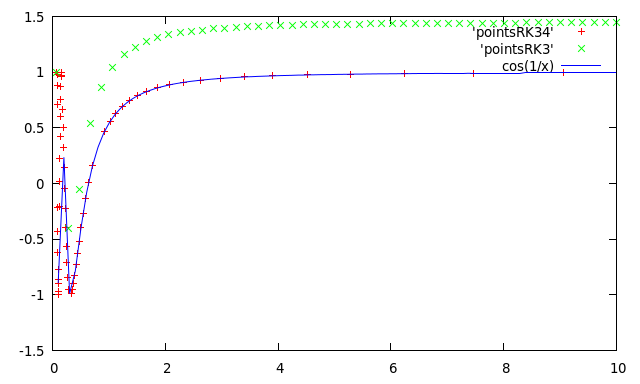
\includegraphics[scale=0.5]{cos1.png}
  							\caption{Pour l'intervalle $[0.08,10]$, seuil de $10^{-5}$, pas de 50}
					\end{figure}
	
					\begin{figure}[!h]
						\centering
  							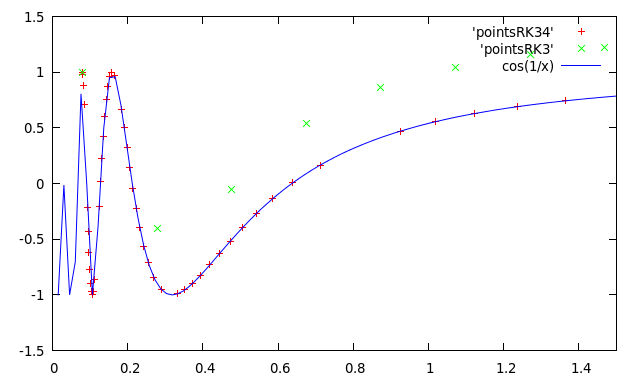
\includegraphics[scale=0.5]{cos2.png}
  							\caption{La même image zommée}
					\end{figure}
					\newpage

					On voit ici clairement les limites de la méthode à pas adaptatif, qui réagit assez mal à ces oscillations aussi violentes.
					La méthode à pas constant est toujours aussi limitée, sauf si l'on se donne un pas très élevé, ce qui n'est pas très optimisé et difficile à prévoir.
					On peut toutefois voir qu'en prenant une erreur de consistance plus faible, la méthode reste correcte :
	
					\begin{figure}[!h]
						\centering
  							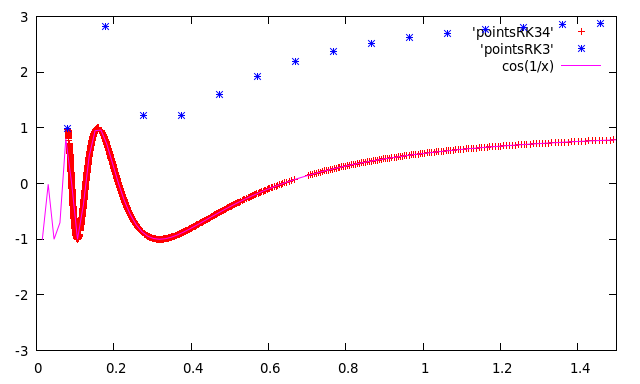
\includegraphics[scale=0.5]{RK350.png}
  							\caption{Pour l'intervalle $[0.08,10]$, seuil à $10^{-10}$, pas de 50}
					\end{figure}
	
					\begin{figure}[!h]
						\centering
  							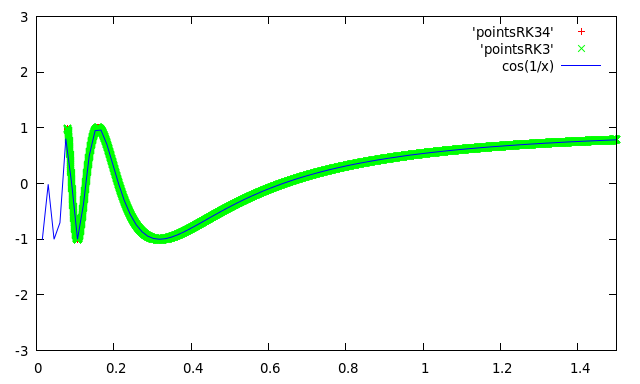
\includegraphics[scale=0.5]{RK3100000.png}
  							\caption{Pour l'intervalle $[0.08,10]$, seuil à $10^{-10}$, pas de 100000}
					\end{figure}
					\newpage

					On remarque ensuite que à partir d'une certaine valeur de $a$ critique, notre courbe se décale complétement de la solution réelle pour un seuil de $10^{-10}$ :
					
					\begin{figure}[!h]
						\centering
  							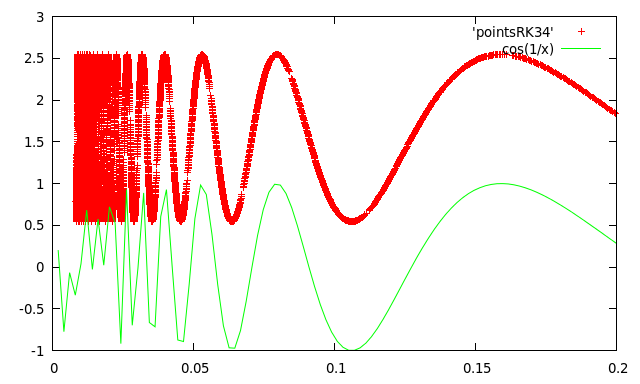
\includegraphics[scale=0.5]{valcritique.png}
  							\caption{Valeur critique à $a = 0.05$ pour RK34}
					\end{figure}
					\newpage

				\subsubsection{Comparaison des résultats}
					Nous avons ici vu que le pas adaptatif garantit une adaptation du pas à l'erreur choisie : si la solution oscille beaucoup, alors il y aura beaucop de points.
					Pour un pas constant, il faut être capable de prévoir ce comportement pour la solution, ce qui n'est pas évident.

			\subsection{Retour aux racines}
				On se donne $f(x,y) = \sqrt{x}y^{2}$.

				\subsubsection{Résolution directe}
					On a donc :

					\[\begin{aligned}
						\frac{dy}{y^{2}} = \sqrt{t}dt
						& \Leftrightarrow \int_{a}^{x} \frac{dy}{y^{2}} =\int_{a}^{x} \sqrt{t}dt \\
						& \Leftrightarrow -\frac{1}{y} = \frac{2}{3}(x\sqrt{x} - a\sqrt{a}) - \frac{1}{y_{0}}\\
						& \Leftrightarrow y(x)=\frac{1}{\frac{2}{3}(a\sqrt{a} - x\sqrt{x}) + \frac{1}{y_{0}}}
					\end{aligned}\]

				\subsubsection{Application de la méthode}
					On choisit $y_0 = 1$.

					\begin{figure}[!h]
						\centering
  							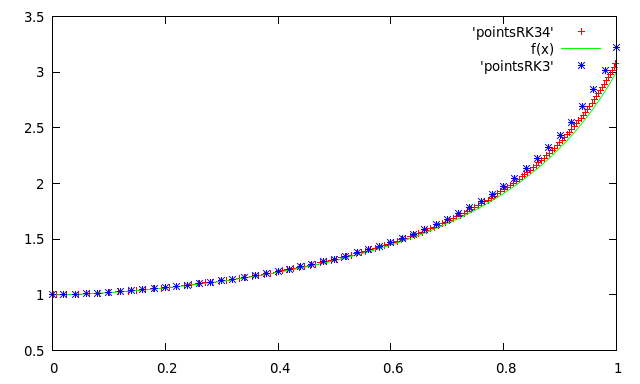
\includegraphics[scale=0.5]{derexemple.png}
  							\caption{Pour l'intervalle $[0,1]$, seuil à $10^{-5}$, pas de 50}
					\end{figure}
					\newpage
					
					\begin{figure}[!h]
						\centering
  							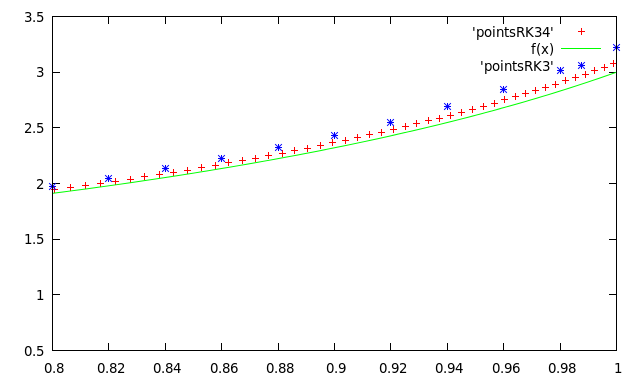
\includegraphics[scale=0.5]{derexemplezoom.png}
  							\caption{La même image zoomée}
					\end{figure}

					\begin{figure}[!h]
						\centering
  							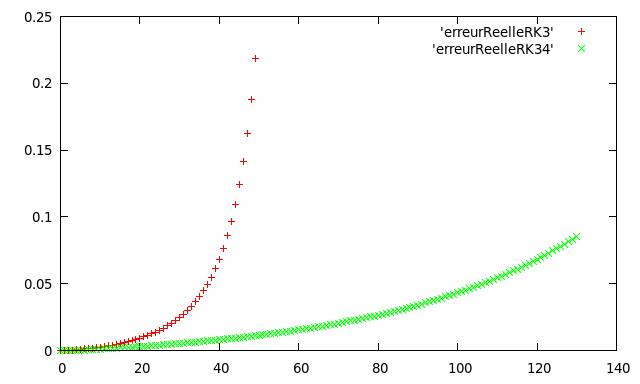
\includegraphics[scale=0.5]{erreurReelleEx5.jpg}
  							\caption{Erreur réelle}
					\end{figure}
					\newpage

			\subsection{Normal}
				Pour retrouver les tables de la loi normale, nous avons décidé de prendre l'exemple $f(x,y) = \frac{1}{\sqrt{2\pi}}e^{-\frac{x^{2}}{2}}$.

				\subsubsection{Application de la méthode}
					On choisit l'intervalle d'étude $[-4,4]$ avec $y_{0} = \Phi(-4)$.

					\begin{figure}[!h]
						\centering
  							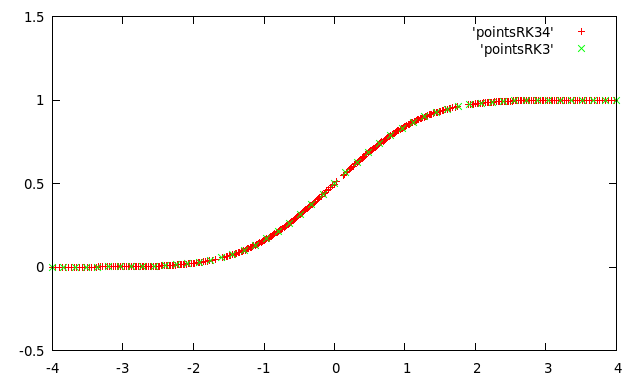
\includegraphics[scale=0.5]{loinormale.png}
  							\caption{Loi normale, seuil de $10^{-5}$, pas de 50 pour la méthode $RK_{3}$}
					\end{figure}
					\newpage

					On retrouve bien le graphe de $\Phi$.
					Les valeurs données par la méthode correspondent à $10^{-3}$ près aux valeurs des tables, ce qui est une bonne approximation.


		\section{Bilan concernant la méthode $RK_{34}$}
			Tout d'abord expliquons les exemple étudiés. 
			Nous avons dans un premier temps décidé de tester nos programmes sur des équations différentielles faciles à résoudre afin de vérifier nos résultats. 
			Ensuite nous nous sommes rendus compte que l'erreur variait si la solution était convergente et divergente. 
			C'est pourquoi nous avons utilisé les cas $f(x,y) = y$ et $f(x,y) = -y$. 
			Par la suite, nous avons voulons étudier le cas dune fonction qui oscillait rapidement, typiquement $cos\left(\frac{1}{x}\right)$. 
			Ensuite , nous avons cherché une équation différentielle qui dépendait des deux paramètres x et y. 
			En dernier lieu, nous avions pour objectif de trouver une application concrète de cette méthode. 
			Nous avons alors eu l'idée de la loi normale.

			Finalement, après étude de plusieurs cas différent, il apparaît que la méthode de résolution de Runge Kutta 34 à pas variable nous donne une meilleure approximation que la méthode de Runge Kutta 3 dans presque tout les cas de figure.
			En plus, elle permet de limiter les calculs en adoptant un pas optimal et s'adapte à la fonction étudiée.
			Si nous avions voulu obtenir les même résultats à pas constant, il aurait fallu trouver le pas vérifiant $\max_{k} \epsilon_{k}(h) < seuil$.

	\chapter*{Conclusion}
	\addcontentsline{toc}{chapter}{Conclusion} % ajouter la conclusion au sommaire
		Ce projet nous a permis d'étudier une méthode de résolution des équations différentielles ordinaires : la méthode $RK_{34}$ à pas adaptatif. 
		Nous avons implémenté cette méthode d'abord en fortran à pas constant, puis à pas variable avec des tableaux dynamique en fortran et en C.
		Après avoir revu notre code afin d'éviter l'utilisation de tableaux dynamiques, notre programme nous a offert à la fois de bonnes approximations des points discrétisés, mais aussi une optimisation en coût et en mémoire lors de l’exécution. 

		Nous avons testé la pertinence de notre programme en comparant nos résultats aux valeurs exactes et nous nous sommes alors rendu compte que ces derniers étaient très proches des valeurs attendues, à l'exception des fonctions admettant des valeurs critiques au voisinage de certains points (par exemple $cos\left(\frac{1}{x}\right)$).
		L'étude de ces exemples de fonctions convergentes, divergentes et oscillantes avec les méthodes $RK_{34}$ et $RK_{3}$ nous a montré l'intérêt du pas adaptatif et ses limites. 

		Tous les deux passionnés par ce sujet, nous avons apprécié ce projet, même s'il a été difficile de s'organiser.
		Nous aurions aimé ajouter certains éléments à ce projet :
		\begin{itemize}
			\item une étude supplémentaire permettant une généralisation de la methode de $RK_{pp'}$, où l'utilisateur pourrait entrer les coefficients lui même;
			\item passer la fonction $f(x,y)$ en paramètre du programme;
			\item diversifier et approfondir les exemples;
			\item généraliser le domaine d'étude au cas $\mathbb{R}^m$.
		\end{itemize}

	\appendix
	\addtocontents{toc}{\protect\setcounter{tocdepth}{0}} % profondeur table des matières annexes
	
	\begin{thebibliography}{9}
	\addcontentsline{toc}{chapter}{Bibliographie} % ajouter la bibliographie au sommaire
	
		\bibitem{Cours 01}
			\emph{Nicolas Forcadel},
			\textit{Cours d'Analyse Numérique},
			Institut National des Sciences Appliquées de Rouen.

		\bibitem{Cours 02}
			\emph{Andre Draux},
			\textit{Cours d'Analyse Numérique},
			Institut National des Sciences Appliquées de Rouen.

		\bibitem{Cours 03}
			\emph{Olivier Mgbra},
			\textit{Cours sur les méthodes de résolution des EDO},
			Youtube.

		\bibitem{Livre 01}
			\emph{Ernst Hairer, Syvert P. N\o rsett, Gerhard Wanner},
			\textit{Solving Ordinary Differential Equations I – Nonstiff Problems},
			Springer, 2008.

		\bibitem{Livre 02}
			\emph{Ernst Hairer, Christian Lubich, Gerhard Wanner},
			\textit{Geometric Numerical Integration – Structure-Preserving Algorithms for Ordinary Differential Equations},
			Springer.
	
		\bibitem{Article 01}
			\emph{John C. Butcher},
			\textit{A history of Runge-Kutta methods},
			Université d'Auckland (Nouvelle Zélande), 1996.

		\bibitem{Lien Internet 01}
			\url{http://showard.sdsmt.edu/Math373/_AppliedNumMethodsText_SMH/RK_History.htm},
			History of Runge-Kutta methods,
			(Valide à la date du 05/03/2014).
	
	\end{thebibliography}

\end{document} % fin du document
